\chapter{Extração de Dados}
\label{cap:Extracao}

Para a extração dos dados para a análise de sentimentos foi criado um
\textit{crawler} ou robô de navegação. Esse robô tem como objetivo a navegação
automática no conteúdo web do Reddit, extraindo os dados referentes a tópicos e
a comentários e persistindo esses em um banco de dados. 

\section{\textit{Crawler}}

O \textit{Crawler} foi escrito na linguagem Java por se tratar de uma linguagem
com uma grande quantidade de bibliotecas disponíveis e também
sua facilidade de implementação. A Figura \ref{fig:crawler} representa a
arquitetura utilizada para desenvolvimento deste software.

\begin{figure}[htbp]
 \centering
 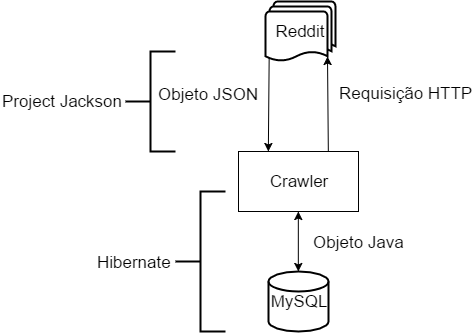
\includegraphics[height=225px]{imagens/arquitetura.png}
 \caption{Arquitetura do \textit{Crawler}}
 \label{fig:crawler}
\end{figure}

A partir de um \textit{link} para um tópico, o software tem como tarefa, a
extração e pesquisa de dados relacionados com o tópico em questão. Isso se faz
da seguinte forma, primeiramente, é enviada uma requisição para o \textit{link}
utilizando o sufixo ``.json'', de forma demonstrada na API, a partir dessa
requisição, o \textit{website} retorna um objeto \ac{JSON}. 

Como o \ac{JSON} possui 68 campos que assim como seus tipos de dados, não se
encontram em nenhuma documentação, foi utilizado o \textit{website}
jsonschema2pojo\footnote{http://www.jsonschema2pojo.org/} para mapear o \ac{JSON} retornado em um
objeto Java. Esse \textit{website} tem como objetivo a conversão de um esquema \ac{JSON} ou o próprio \ac{JSON} para um \ac{POJO} ou Os Singelos Clássicos Objetos Java, permitindo
o \textit{download} da classe para utilização, já com as anotações
``@JsonProperty'' utilizadas na biblioteca Jackson. Este objeto disponibilizado a
partir do \textit{website} foi renomeado para \textit{RedditPost} e adicionado
ao código fonte da aplicação.

A anotação ``@JsonProperty'' é relativa ao
mapeamento do objeto Java com relação ao \ac{JSON} e nos permite com
intermédio da classe \textit{Object Mapper} instanciar o objeto
\textit{RedditPost} a partir de um objeto \textit{String} em formato \ac{JSON}. 

\begin{lstlisting}
RedditPost post = objectMapper.readValue(iteratorPost.get("data").toString(),
RedditPost.class);
\end{lstlisting}

Utilizando o método \textit{readValue} que tem como retorno um \textit{Object},
é informado um objeto \textit{String}, neste caso
\textit{``iteratorPost.get("data").toString()"} e uma classe mapeada, neste caso
\textit{RedditPost}.

Porém, para o correto funcionamento, deve ser feita a seguinte mudança: O campo
\textit{edited} representando se foi editado o comentário, retornado no
\ac{JSON} apresenta um tipo de dado ambíguo aonde que caso o comentário não tenha sido editado, ele apresenta o valor \textit{booleano} de \textit{false}, porém, ao ter sido editado, ele apresenta
seu valor em um formato decimal. Este e demais objetos que apresentavam o tipo
de dado de forma ambígua foram transformados em objetos \textit{String}.


A partir deste objeto Java, foi utilizado o \textit{framework} Hibernate para a
criação do banco de dados, assim como persistência destes. Através da anotação
``@Entity'', adicionada também na classe RedditPost. O Hibernate mapeia essa
entidade junto ao banco de dados, neste caso, MySQL.

Para criação das tabelas do banco de dados, foi utilizada a propriedade
\textit{hibernate.hbm2ddl.auto} do Hibernate. Essa propriedade quando
instânciada uma nova sessão do \textit{framework} no Java executa as seguintes
ações dependendo de seus valores informados:


\begin{itemize}
  \item \textit{validate}: Não efetua mudanças no banco de dados, somente
  valida.
  \item \textit{update}: Atualiza o esquema do banco de dados conforme os
  objetos mapeados na camada Java.
  \item \textit{create}: Cria o esquema contendo tabelas e campos a partir dos
  objetos Java, destruindo dados anteriores.
  \item \textit{create-drop}: Cria o esquema da mesma que o \textit{create},
  porém, ao termino da sessão, remove o esquema criado.
\end{itemize}

No primeiro momento, a propriedade obteve o valor \textit{create}, para fins de
criação e validação do esquema criado e após isso, foi informado \textit{update}
como seu valor para tornar reflexo as alterações feitas na camada Java.

Portanto, a execução do \textit{Crawler} funciona da seguinte forma, é enviada
uma requisição para o \textit{website} através da URL do tópico em questão com o
sufixo ``\textit{.json}'' no final. O \textit{website} retorna um
\textit{JSON} com os dados referentes ao tópico solicitado e aos comentários
deste tópico. Este objeto \ac{JSON} é convertido em um \ac{POJO} através da
biblioteca Jackson e persistida no banco de dados através do \textit{framework}
Hibernate. Como a API do Reddit possui uma restrição do número de comentários
disponibilizados, são efetuadas novas requisições para a seção \textit{``more''}
disponível no \ac{JSON} de retorno.

